\documentclass{article}
\usepackage{graphicx}

\title{Case Study 2 - The Board Meeting - Sam}
\author{Graham Pellegrini}
\date{}

\begin{document}

\maketitle

\section{Plan to Manage Computer Sales}

\subsection{a. The first 48 hours of running the business} 
\begin{itemize}
    \item \textbf(No immediate changes) - I would not make any immediate changes to the business.
    \item \textbf{Meeting with Steve} - Discuss the current state of the business and actions being taken to align with the business vision.
    \item \textbf{Meeting with the team} Begin establishing rapport and prioritizing communication for feedback with the team.
    \item \textbf{Begin Analyzes} Spend time reviewing sales metrics, reviews, and market state.
\end{itemize}


\subsection{b. The first week of running the business}
\begin{itemize}
    \item \textbf{Team Meetings} - Meet with department heads to understand challenges and gather ideas.
    \item \textbf{Observe the day to day sales} - Observe daily sales to assess the current state of the business and team operations.
    \item \textbf{Identify minor adjustments} - Identify minor adjustments for positive impact without making too many changes quickly.
\end{itemize}


\subsection{c. The first month of running the business}
\begin{itemize}
    \item \textbf{Short-term goals} - Define measurable goals to assess team operations and identify issues.
    \item \textbf{Improvement Plan} - Create a plan to drive team enthusiasm, possibly investing in training and resources.
    \item \textbf{Meetings with Computer Engineering department} - Foster unity and teamwork by celebrating departmental achievements.
\end{itemize}


\subsection{d. The first six months of running the business}
\begin{itemize}
    \item \textbf{Develop Talent} - Form a talent group to rapidly implement ideas and respond to market trends.
    \item \textbf{Strengthen customer relationships} - Ensure best customer service through training and new strategies.
    \item \textbf{Streamline operations} - Identify inefficiencies and work towards a more efficient business model.
\end{itemize}


\subsection{e. The first year of running the business}
\begin{itemize}
    \item \textbf{Avoid Stagnation} - Keep the team motivated and driven towards set goals.
    \item \textbf{Market Leader} - Maintain market leader status by keeping up with trends.
    \item \textbf{Possible online store} - Explore the possibility of an online store to reach a wider audience.
    \item \textbf{Personal Managering Development} - Continue personal development to enhance business acumen.
    \item \textbf{Meetings with the board} - Promote openness and transparency in board meetings.
\end{itemize}


\subsection{f.What leadership style should Sam employ?}

\subsection{f. What leadership style should Sam employ?}
Sam should employ a \textbf{democratic leadership style} this will:
\begin{itemize}
    \item Involve the team in decision-making while retaining final responsibility. When engaged in the decision-making process, employees are more likely to be motivated and committed to the success of the business.
    \item Foster an enviroment for inspiring ideas. The openess of the democratic leadership style will allow for the team to share their ideas and contribute to the growth of the business.
    \item Delegate tasks between team members, ensuring Sam is not overwhelmed with the day-to-day operations and can focus on the management of the business.
\end{itemize}


\subsection{g. How should he liaise with Julie and the Computer Engineering Division?}
- The two departements are seperate in their operations. \\
- So colobaration is more trivial than functional. \\

\begin{itemize}
    \item \textbf{Cross departmental meetings} - Sam and Julie can understand each other's operations and the reason behind decisions taken.
    \item \textbf{Delegated meetings} - Meetings can be delegated to department heads that would then report back to Sam and Julie. This would also alow word to flow between the two departments.
    \item \textbf{celebrate achievements} - Building on the flow of word between the two departments, Sam and Julie can celebrate departmental achievements. For example by hanging a poster in the break room or sending out a company wide email. This would create a sense of unity and teamwork between the two departments.
    \item \textbf{Departemental Dissagreeements} - If disagreements arise between the two departments the only level it should be escalated to is at the board level and should not trickle down to the team level.
\end{itemize}


\subsection{h. What are your first requests going to be to the board?}

\begin{itemize}
    \item \textbf{Capital Investment} I would like to request a capital investment in training or resources where the team will benefit also on a personal level. This would drive enthusiasm to the team and allow them to feel more valued. \\
    \item \textbf{Online Store} I would like to explore the possibility of an online store. This would allow us to reach a wider audience and possibly bring in more revenue. However, keeping in mind the challenges and risks that have kept us from doing so in the past. \\
    \item \textbf{Personal Development} I am open to the fact that I will make mistakes. So I wish to be to properly learn from them with guidance rather than solutions from Steve. \\
\end{itemize}

\pagebreak
\section{The Software Bug}

\subsection{i. Warning Julie directly}
\textbf{Advantages:} \\
- Bug likely fixed before product launch. \\
- Establishes trust and teamwork between Sam and Julie. \\

\textbf{Disadvantages:} \\
- Julie may see it as a threat to her position. \\
- Sam may be seen as a snitch by the Computer Engineering Division. \\

\subsection{j. Not warning Julie or anyone}
\textbf{Advantages:} \\
- Sam avoids confrontation with Julie. \\
- Opportunity for Sam to prove leadership. \\

\textbf{Disadvantages:} \\
- Product launch likely to fail, harming Julie's division. \\

\subsection{k. Warning the board of the problem in the next board meeting}
\textbf{Advantages:} \\
- Board can decide on product launch. \\
- Shows Sam's value and willingness to help beyond his responsibilities. \\

\textbf{Disadvantages:} \\
- Julie may see it as a threat. \\
- Could damage Sam and Julie's relationship, affecting departmental cooperation. \\
- Board may see it as a betrayal of trust. \\

\subsection{l. After considering the advantages and disadvantages, what do you think you should do?}
Warn Julie directly. Approach her sincerely and respectfully, explaining the situation and repercussions. This allows Julie to fix the bug before the product launch. In the next board meeting, Sam should highlight the resolution, commend Julie, and demonstrate his broader business perspective.

\pagebreak

\begin{figure}[h]
    \centering
    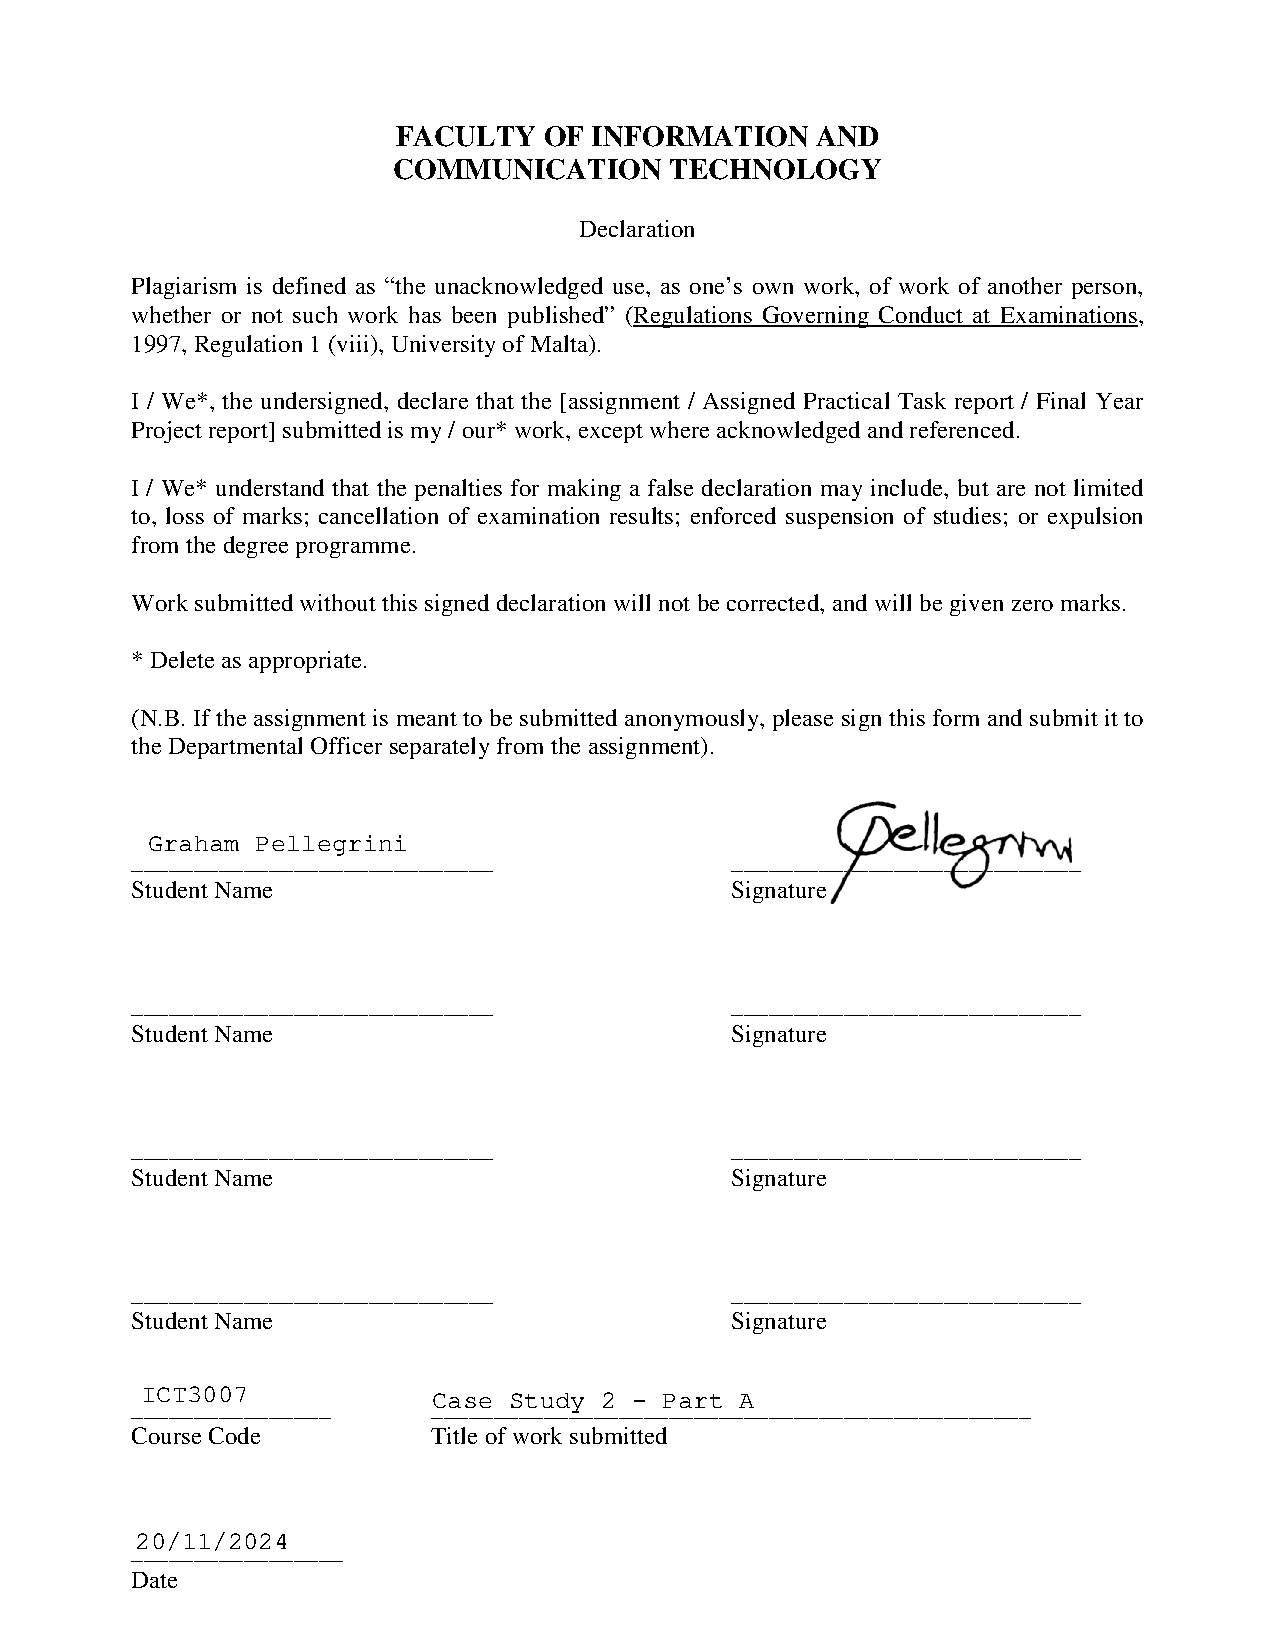
\includegraphics[width=1.2\textwidth]{PlagiarismForm_PartA_SAM.pdf}
    \caption{Plagerism Form}
\end{figure}

\end{document}